\documentclass[a4paper,twoside,onecolumn,openany,article,10pt]{memoir}
\usepackage{xeCJK}
\usepackage{url}
\usepackage{hyperref}
\usepackage{amsmath}
\usepackage{amssymb}
\usepackage{amsthm}
\usepackage{enumerate}
\usepackage{algorithm}
\usepackage{algorithmicx}
\usepackage{algpseudocode}
\usepackage{ascmac}
\usepackage{tikz}
\usepackage{ulem}
%\usepackage{stix}
\defaultfontfeatures{Ligatures=TeX}

\setCJKmainfont[BoldFont=Noto Sans CJK JP]{Noto Serif CJK JP}
\setCJKsansfont{Noto Sans CJK JP}
%\setCJKmonofont{Inconsolata}

\newtheorem{theorem}{定理}
\theoremstyle{remark}
\newtheorem{remark}{\textbf{余談}}


\setmainfont{DejaVu Serif}
%\setsansfont{URW Gothic}
\setmonofont{Inconsolata}

\usepackage{listings}

%\renewcommand{\algorithmcfname}{アルゴリズム}



\settrimmedsize{\stockheight}{\stockwidth}{*}

%\setlrmarginsandblock{1.5in}{1in}{*}
\setlrmarginsandblock{1.2in}{1.2in}{*}
\setulmarginsandblock{1.2in}{1.5in}{*}
\setheadfoot{20mm}{15mm}

%\newlength{\linespace}
%\setlength{\linespace}{\baselineskip}
%\setlength{\headheight}{\onelineskip}
%\setlength{\headsep}{\linespace}
%\addtolength{\headsep}{-\topskip}

%\setlength{\footskip}{\onelineskip}
%\setlength{\footnotesep}{\onelineskip}

\checkandfixthelayout

\counterwithout{section}{chapter}
\setsecnumdepth{subsubsection}


\title{アルゴリズムとデータ構造~プログラミング演習~二分探索}
\date{2017年6月13日}
\author{森~立平 \texttt{mori@c.titech.ac.jp}}

\begin{document}
\maketitle


\noindent
今日の目標
\begin{itemize}
\item 二分探索のプログラムを書けるようになる。
\item 二分探索を使いこなせるようになる。
\end{itemize}

\noindent
今日の主な課題(提出締切は授業終了時)
\begin{enumerate}
\item 二分探索のプログラムを完成させる。
\item 二分探索を用いてより難しい問題を解く。
\end{enumerate}

\noindent
今日のワークフロー
\begin{enumerate}
\item この資料をよく読み二分探索の考え方及び、そのC言語プログラムについて理解する。
\item \ref{sec:assign}章に書いてある課題に取り組む.
\item 教員かTAに課題提出.
\end{enumerate}

\section{はじめに}
ウェブブラウザで \url{https://github.com/ryuhei-mori/2017ad} にアクセスして「プログラミング演習のルール」を\textbf{必ず読む}こと。
他にもこの資料やC言語のプログラムが置いてある。


\section{二分探索について}
二分探索とはソートされている配列から、与えられた数$x$以上の最小の数及びそのインデックスをもとめるアルゴリズムである。
例で説明する。次の長さ12のソートされている配列について、$k=17$以上の最小の数をもとめたいとする。

\begin{center}
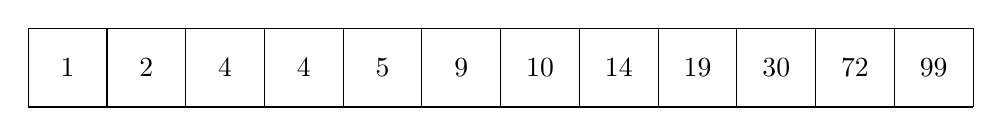
\begin{tikzpicture}
\draw[black] (0,0) grid (12,1);
\node at (0.5,0.5) {1};
\node at (1.5,0.5) {2};
\node at (2.5,0.5) {4};
\node at (3.5,0.5) {4};
\node at (4.5,0.5) {5};
\node at (5.5,0.5) {9};
\node at (6.5,0.5) {10};
\node at (7.5,0.5) {14};
\node at (8.5,0.5) {19};
\node at (9.5,0.5) {30};
\node at (10.5,0.5) {72};
\node at (11.5,0.5) {99};
\end{tikzpicture}
\end{center}
%
最初に配列の真ん中にある要素について$k=17$以上かどうかチェックする。
%
\begin{center}
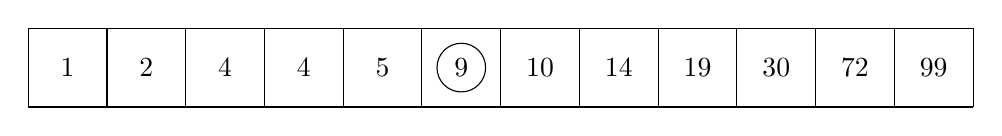
\begin{tikzpicture}
\draw[black] (0,0) grid (12,1);
\node at (0.5,0.5) {1};
\node at (1.5,0.5) {2};
\node at (2.5,0.5) {4};
\node at (3.5,0.5) {4};
\node at (4.5,0.5) {5};
\node[circle,draw] at (5.5,0.5) {9};
\node at (6.5,0.5) {10};
\node at (7.5,0.5) {14};
\node at (8.5,0.5) {19};
\node at (9.5,0.5) {30};
\node at (10.5,0.5) {72};
\node at (11.5,0.5) {99};
\end{tikzpicture}
\end{center}
%
9は17よりも小さいので、この9よりも右にある要素からなる配列について$k=17$以上の最小の数をもとめればよい。
%
\begin{center}
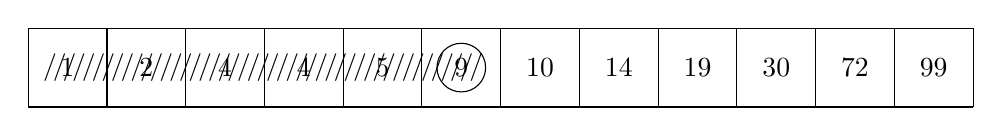
\begin{tikzpicture}
\draw[black] (0,0) grid (12,1);
\node at (0.5,0.5) {1};
\node at (1.5,0.5) {2};
\node at (2.5,0.5) {4};
\node at (3.5,0.5) {4};
\node at (4.5,0.5) {5};
\node[circle,draw] at (5.5,0.5) {9};
\node at (6.5,0.5) {10};
\node at (7.5,0.5) {14};
\node at (8.5,0.5) {19};
\node at (9.5,0.5) {30};
\node at (10.5,0.5) {72};
\node at (11.5,0.5) {99};
\node at (3.0,0.5) {\xout{~\hspace{150pt}~}};
\end{tikzpicture}
\end{center}
%
残りの要素の中から真ん中の要素について$k=17$以上かどうかチェックする。
%
\begin{center}
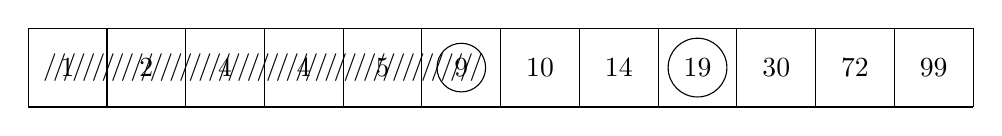
\begin{tikzpicture}
\draw[black] (0,0) grid (12,1);
\node at (0.5,0.5) {1};
\node at (1.5,0.5) {2};
\node at (2.5,0.5) {4};
\node at (3.5,0.5) {4};
\node at (4.5,0.5) {5};
\node[circle,draw] at (5.5,0.5) {9};
\node at (6.5,0.5) {10};
\node at (7.5,0.5) {14};
\node[circle,draw] at (8.5,0.5) {19};
\node at (9.5,0.5) {30};
\node at (10.5,0.5) {72};
\node at (11.5,0.5) {99};
\node at (3.0,0.5) {\xout{~\hspace{150pt}~}};
\end{tikzpicture}
\end{center}
%
19は17以上なので、この19を含む19よりも左側にある要素からなる配列について $k=17$以上の最小の数をもとめればよい。
%
\begin{center}
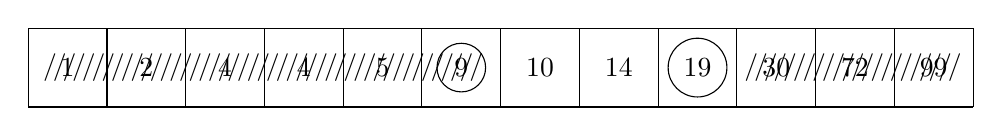
\begin{tikzpicture}
\draw[black] (0,0) grid (12,1);
\node at (0.5,0.5) {1};
\node at (1.5,0.5) {2};
\node at (2.5,0.5) {4};
\node at (3.5,0.5) {4};
\node at (4.5,0.5) {5};
\node[circle,draw] at (5.5,0.5) {9};
\node at (6.5,0.5) {10};
\node at (7.5,0.5) {14};
\node[circle,draw] at (8.5,0.5) {19};
\node at (9.5,0.5) {30};
\node at (10.5,0.5) {72};
\node at (11.5,0.5) {99};
\node at (3.0,0.5) {\xout{~\hspace{150pt}~}};
\node at (10.5,0.5) {\xout{~\hspace{70pt}~}};
\end{tikzpicture}
\end{center}
%
残りの要素から真ん中の要素を調べる。
%
\begin{center}
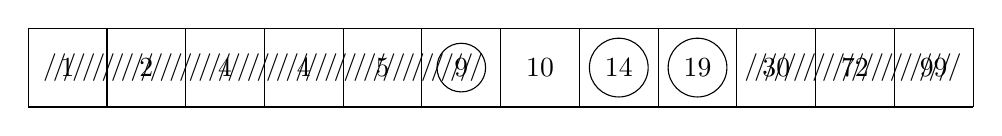
\begin{tikzpicture}
\draw[black] (0,0) grid (12,1);
\node at (0.5,0.5) {1};
\node at (1.5,0.5) {2};
\node at (2.5,0.5) {4};
\node at (3.5,0.5) {4};
\node at (4.5,0.5) {5};
\node[circle,draw] at (5.5,0.5) {9};
\node at (6.5,0.5) {10};
\node[circle,draw] at (7.5,0.5) {14};
\node[circle,draw] at (8.5,0.5) {19};
\node at (9.5,0.5) {30};
\node at (10.5,0.5) {72};
\node at (11.5,0.5) {99};
\node at (3.0,0.5) {\xout{~\hspace{150pt}~}};
\node at (10.5,0.5) {\xout{~\hspace{70pt}~}};
\end{tikzpicture}
\end{center}
%
14 は 17よりも小さいので、この14よりも右側だけを調べればよい。
%
\begin{center}
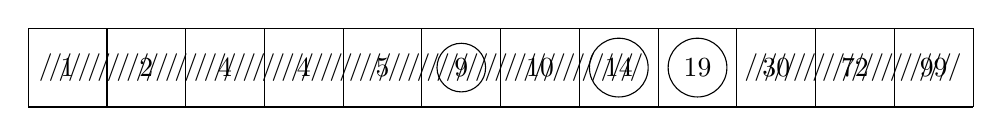
\begin{tikzpicture}
\draw[black] (0,0) grid (12,1);
\node at (0.5,0.5) {1};
\node at (1.5,0.5) {2};
\node at (2.5,0.5) {4};
\node at (3.5,0.5) {4};
\node at (4.5,0.5) {5};
\node[circle,draw] at (5.5,0.5) {9};
\node at (6.5,0.5) {10};
\node[circle,draw] at (7.5,0.5) {14};
\node[circle,draw] at (8.5,0.5) {19};
\node at (9.5,0.5) {30};
\node at (10.5,0.5) {72};
\node at (11.5,0.5) {99};
\node at (4.0,0.5) {\xout{~\hspace{210pt}~}};
\node at (10.5,0.5) {\xout{~\hspace{70pt}~}};
\end{tikzpicture}
\end{center}
19だけが残ったので19が解である。

\section{二分探索のプログラム}
\if0
二分探索というアルゴリズムを理解するのは簡単だが、プログラムを書くのは少しだけ難しい。
例えば、
\begin{center}
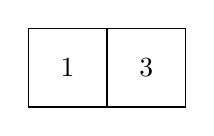
\begin{tikzpicture}
\draw[black] (0,0) grid (2,1);
\node at (0.5,0.5) {1};
\node at (1.5,0.5) {3};
\end{tikzpicture}
\end{center}
という長さ2の配列から$k=2$以上の最小の数をもとめる場合、最初に3を調べると、$3\ge k=2$のため、3を含む3より左側にある要素を調べることになる。
そうすると、次のステップでまた3を調べることになり無限ループに陥いる。
また、
\begin{center}
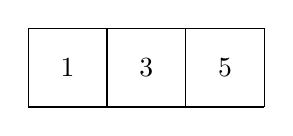
\begin{tikzpicture}
\draw[black] (0,0) grid (3,1);
\node at (0.5,0.5) {1};
\node at (1.5,0.5) {3};
\node at (2.5,0.5) {5};
\end{tikzpicture}
\end{center}
という長さ3の配列から$k=6$以上の最小の数をもとめる。
\fi

長さ$n$の配列について$k$以上の最小の要素を出力するC言語プログラムは次のようになる。
ただし$k$以上の要素が無い場合は、``NO''を出力する。

\begin{lstlisting}[basicstyle=\ttfamily\small,showstringspaces=false,language=C,frame=single]
int lb, ub;
lb = -1;
ub = n;

while(ub - lb > l) {
  int mid = (lb + ub) / 2;
  if(A[mid] >= k){
    ub = mid;
  }
  else{
    lb = mid;
  }
}

if(ub == n) {
   printf("NO\n");
}
else {
  printf("The answer is %d\n", A[ub]);
}
\end{lstlisting}
変数\texttt{lb}と\texttt{ub}の意味は
\begin{itemize}
\item 変数\texttt{lb}は\texttt{A[i] < k}を確認した最大の\texttt{i}
\item 変数\texttt{ub}は\texttt{A[i] >= k}を確認した最小の\texttt{i}
\end{itemize}
である。便宜上\texttt{A[-1]}をマイナス無限、\texttt{A[n]}をプラス無限と解釈しているので、\texttt{lb = -1}、\texttt{ub = n}と初期化する。
実際にプログラムの中でアクセスされるのは\texttt{A[0]}から\texttt{A[n-1]}までなので心配はいらない。
もしも\texttt{ub == lb + 1}であれば、\texttt{A[ub]}が\texttt{A[i] >= k}を満たす最小の値である。
\texttt{ub - lb > 1}の場合、\texttt{while}ループの中でまず\texttt{mid = (lb + ub) / 2} を計算する(小数点以下切り捨てとなる)。
このとき、\texttt{lb < mid \&\& mid < ub} が満たされることに注意する。
\texttt{A[mid] >= k} が満たされていれば \texttt{ub = mid} に更新し、
満たされていなければ \texttt{lb = mid} と更新する。
ここで、\texttt{ub - lb} は\textbf{必ず減少する}ので無限ループに陥いることはない。
前節の例に対して上記のプログラムお実行した場合に\texttt{lb}と\texttt{ub}がどのように更新されるかを下の図で示す。

\begin{center}
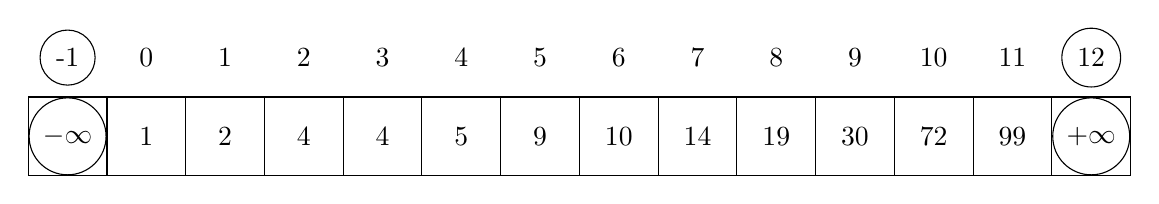
\begin{tikzpicture}
\draw[black] (-1,0) grid (13,1);
\node[circle,draw] at (-0.5,0.5) {$-\infty$};
\node at (0.5,0.5) {1};
\node at (1.5,0.5) {2};
\node at (2.5,0.5) {4};
\node at (3.5,0.5) {4};
\node at (4.5,0.5) {5};
\node at (5.5,0.5) {9};
\node at (6.5,0.5) {10};
\node at (7.5,0.5) {14};
\node at (8.5,0.5) {19};
\node at (9.5,0.5) {30};
\node at (10.5,0.5) {72};
\node at (11.5,0.5) {99};
\node[circle,draw] at (12.5,0.5) {$+\infty$};
\node[circle,draw] at (-0.5,1.5) {-1};
\node at (0.5,1.5) {0};
\node at (1.5,1.5) {1};
\node at (2.5,1.5) {2};
\node at (3.5,1.5) {3};
\node at (4.5,1.5) {4};
\node at (5.5,1.5) {5};
\node at (6.5,1.5) {6};
\node at (7.5,1.5) {7};
\node at (8.5,1.5) {8};
\node at (9.5,1.5) {9};
\node at (10.5,1.5) {10};
\node at (11.5,1.5) {11};
\node[circle,draw] at (12.5,1.5) {12};
\end{tikzpicture}
\end{center}

\begin{center}
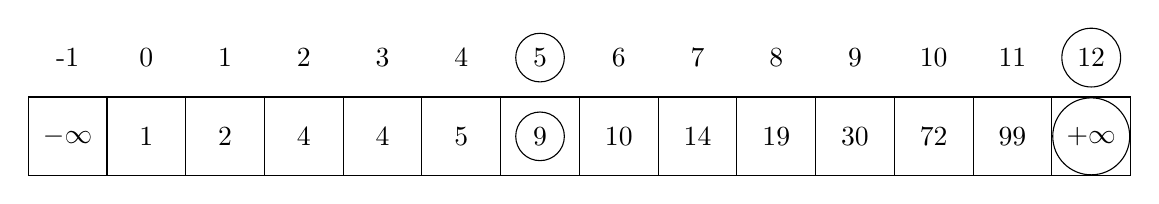
\begin{tikzpicture}
\draw[black] (-1,0) grid (13,1);
\node at (-0.5,0.5) {$-\infty$};
\node at (0.5,0.5) {1};
\node at (1.5,0.5) {2};
\node at (2.5,0.5) {4};
\node at (3.5,0.5) {4};
\node at (4.5,0.5) {5};
\node[circle,draw] at (5.5,0.5) {9};
\node at (6.5,0.5) {10};
\node at (7.5,0.5) {14};
\node at (8.5,0.5) {19};
\node at (9.5,0.5) {30};
\node at (10.5,0.5) {72};
\node at (11.5,0.5) {99};
\node[circle,draw] at (12.5,0.5) {$+\infty$};
\node at (-0.5,1.5) {-1};
\node at (0.5,1.5) {0};
\node at (1.5,1.5) {1};
\node at (2.5,1.5) {2};
\node at (3.5,1.5) {3};
\node at (4.5,1.5) {4};
\node[circle,draw] at (5.5,1.5) {5};
\node at (6.5,1.5) {6};
\node at (7.5,1.5) {7};
\node at (8.5,1.5) {8};
\node at (9.5,1.5) {9};
\node at (10.5,1.5) {10};
\node at (11.5,1.5) {11};
\node[circle,draw] at (12.5,1.5) {12};
\end{tikzpicture}
\end{center}

\begin{center}
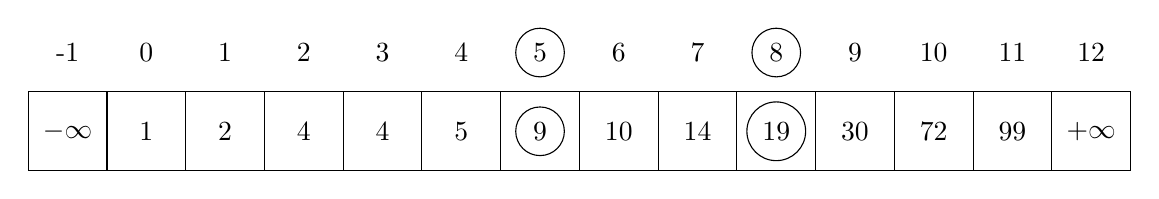
\begin{tikzpicture}
\draw[black] (-1,0) grid (13,1);
\node at (-0.5,0.5) {$-\infty$};
\node at (0.5,0.5) {1};
\node at (1.5,0.5) {2};
\node at (2.5,0.5) {4};
\node at (3.5,0.5) {4};
\node at (4.5,0.5) {5};
\node[circle,draw] at (5.5,0.5) {9};
\node at (6.5,0.5) {10};
\node at (7.5,0.5) {14};
\node[circle,draw] at (8.5,0.5) {19};
\node at (9.5,0.5) {30};
\node at (10.5,0.5) {72};
\node at (11.5,0.5) {99};
\node at (12.5,0.5) {$+\infty$};
\node at (-0.5,1.5) {-1};
\node at (0.5,1.5) {0};
\node at (1.5,1.5) {1};
\node at (2.5,1.5) {2};
\node at (3.5,1.5) {3};
\node at (4.5,1.5) {4};
\node[circle,draw] at (5.5,1.5) {5};
\node at (6.5,1.5) {6};
\node at (7.5,1.5) {7};
\node[circle,draw] at (8.5,1.5) {8};
\node at (9.5,1.5) {9};
\node at (10.5,1.5) {10};
\node at (11.5,1.5) {11};
\node at (12.5,1.5) {12};
\end{tikzpicture}
\end{center}

\begin{center}
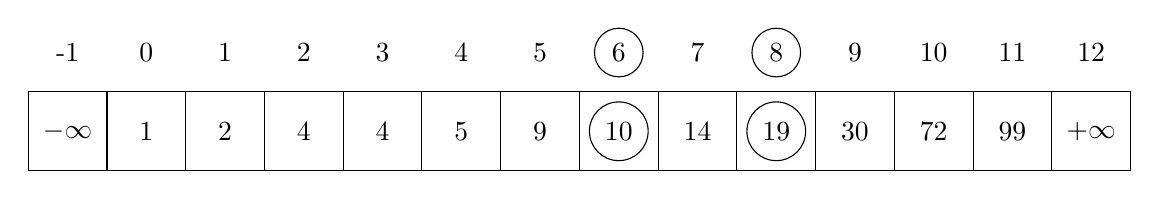
\begin{tikzpicture}
\draw[black] (-1,0) grid (13,1);
\node at (-0.5,0.5) {$-\infty$};
\node at (0.5,0.5) {1};
\node at (1.5,0.5) {2};
\node at (2.5,0.5) {4};
\node at (3.5,0.5) {4};
\node at (4.5,0.5) {5};
\node at (5.5,0.5) {9};
\node[circle,draw] at (6.5,0.5) {10};
\node at (7.5,0.5) {14};
\node[circle,draw] at (8.5,0.5) {19};
\node at (9.5,0.5) {30};
\node at (10.5,0.5) {72};
\node at (11.5,0.5) {99};
\node at (12.5,0.5) {$+\infty$};
\node at (-0.5,1.5) {-1};
\node at (0.5,1.5) {0};
\node at (1.5,1.5) {1};
\node at (2.5,1.5) {2};
\node at (3.5,1.5) {3};
\node at (4.5,1.5) {4};
\node at (5.5,1.5) {5};
\node[circle,draw] at (6.5,1.5) {6};
\node at (7.5,1.5) {7};
\node[circle,draw] at (8.5,1.5) {8};
\node at (9.5,1.5) {9};
\node at (10.5,1.5) {10};
\node at (11.5,1.5) {11};
\node at (12.5,1.5) {12};
\end{tikzpicture}
\end{center}

\begin{center}
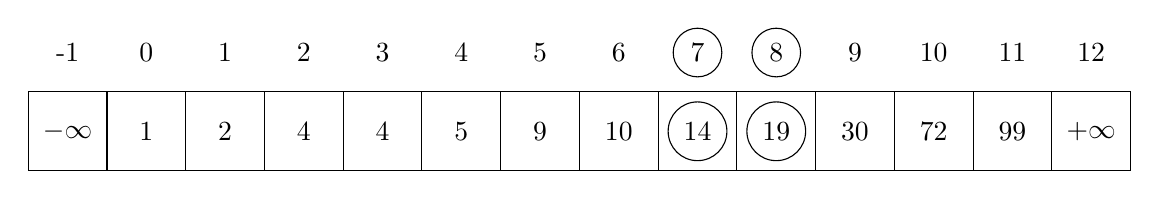
\begin{tikzpicture}
\draw[black] (-1,0) grid (13,1);
\node at (-0.5,0.5) {$-\infty$};
\node at (0.5,0.5) {1};
\node at (1.5,0.5) {2};
\node at (2.5,0.5) {4};
\node at (3.5,0.5) {4};
\node at (4.5,0.5) {5};
\node at (5.5,0.5) {9};
\node at (6.5,0.5) {10};
\node[circle,draw] at (7.5,0.5) {14};
\node[circle,draw] at (8.5,0.5) {19};
\node at (9.5,0.5) {30};
\node at (10.5,0.5) {72};
\node at (11.5,0.5) {99};
\node at (12.5,0.5) {$+\infty$};
\node at (-0.5,1.5) {-1};
\node at (0.5,1.5) {0};
\node at (1.5,1.5) {1};
\node at (2.5,1.5) {2};
\node at (3.5,1.5) {3};
\node at (4.5,1.5) {4};
\node at (5.5,1.5) {5};
\node at (6.5,1.5) {6};
\node[circle,draw] at (7.5,1.5) {7};
\node[circle,draw] at (8.5,1.5) {8};
\node at (9.5,1.5) {9};
\node at (10.5,1.5) {10};
\node at (11.5,1.5) {11};
\node at (12.5,1.5) {12};
\end{tikzpicture}
\end{center}

最終的に\texttt{ub == 8}となる。

\if0
%このプログラムの中で実質的な計算をしている箇所は次の5行である。
%\begin{lstlisting}[basicstyle=\ttfamily\small,showstringspaces=false,language=C,frame=single]
%while(ub - lb > l) {
%  int mid = (lb + ub) / 2;
%  if(A[mid] >= k) ub = mid;
%  else lb = mid;
%}
%\end{lstlisting}
%この5行が実行されたあと(\texttt{while}ループを抜けたあと)、\texttt{ub == lb + 1} が満たされ、その値は\texttt{A[0], A[1], ... A[n-1]}の中で$k$以上の最小の値に対応するインデックスである。
%もしも$k$以上の値が存在しない場合は\texttt{ub}の値は変化しない。


二分探索を書く上で\textbf{一番}気をつけなければいけないことは、無限ループに陥いることである。
そのためには
\begin{center}
\textbf{一回のループで必ず\texttt{l}が大きくなる、もしくは\texttt{r}が小さくなること}
\end{center}
を確認する必要がある。
\texttt{int m = (l + r) / 2;} と計算したとき、\texttt{m}の値は必ず\texttt{l}以上、\texttt{r}未満である(\texttt{r > l} が満たされていることと\texttt{z / 2} が切り下げ$\lfloor \mathtt{z} / 2\rfloor$であることに注意)。
よって\texttt{r = m;}は必ず\texttt{r}を小さくするし、\texttt{l = m + 1;} は必ず\texttt{l}を大きくする。
一回のループで必ず\texttt{r - l}は減少するので無限ループに陥ることはない。

次に上記のプログラムが正しく動作することを示す。
プログラムの\texttt{while}ループを抜けたとき、
\fi

\if0
\section{二分探索の時間計算量}
二分探索の時間計算量について考えよう。
\texttt{while}ループの中の処理は定数時間で可能なので、\texttt{while}ループが繰り返される回数を数えればよい。
簡単のために$n=2^m-1$と仮定する($m$は自然数)。
すると、\texttt{ub - lb}は\texttt{while}ループに入る前は\texttt{n+1}つまり$2^m$になる。
また、
\fi


\section{より高度な二分探索の使い方}
二分探索はソートされた配列から値を探すという目的以外にも使用することができる。
ソートされた配列の代わりに単調な二値関数$p\colon \{0,1,2,\dotsc,n-1\}\to\{0,1\}$について考えよう。
ここで$p$が単調というのは$p(i)\ge p(i-1)$が$i=1,2,\dotsc,n-1$について満たされるという意味である。
このような$p$について
\begin{center}
$p(i) = 1$を満たす最小の$i\in\{0,1,2,\dotsc,n-1\}$をもとめよ
\end{center}
という問題を二分探索で解くことができる。
具体的には前節のプログラムのうち5行目からの9行を次のように変更すればよい。
\begin{lstlisting}[basicstyle=\ttfamily\small,showstringspaces=false,language=C,frame=single]
while(ub - lb > l) {
  int mid = (lb + ub) / 2;
  if(p(mid)){
    ub = mid;
  }
  else{
    lb = mid;
  }
}
\end{lstlisting}
実際に変更したのはこの中の3行目の\texttt{if}文の条件だけである。
この考え方を用いると、上記の問題について非常に大きな$n$に対しても現実的な時間で解くことができる。

\section{課題}\label{sec:assign}
以下の問題についてプログラムを書け。
用意されている入力


%\clearpage
\subsection{配列の二分探索 $\bigstar$}
\begin{itembox}[l]{問題文}
単調非減少数列$a_0, a_1,\dotsc, a_{n-1}$と整数$k$について、$a_x\ge k$となる最小の整数$x$を求めよ。
ただし、そのような$x$が存在しないときは$x=n$とする。
\end{itembox}

\begin{itembox}[l]{入力制約}
$1\le n\le 10^5$\\
$1\le k\le 10^9$\\
$1\le a_i\le 10^9$,\hspace{2em} $i\in\{0,1,\dotsc,n-1\}$\\
$a_i\le a_{i+1}$,\hspace{2em} $i\in\{0,1,\dotsc,n-2\}$
\end{itembox}

\begin{itembox}[l]{入力}
$n~k$\\
$a_0~a_1 \dotsb a_{n-1}$
\end{itembox}

\begin{itembox}[l]{出力}
$x$
\end{itembox}

\begin{itembox}[l]{サンプル1}
入力:
\begin{verbatim}
12 17
1 2 4 4 5 9 10 14 19 30 72 99
\end{verbatim}
出力:
\begin{verbatim}
8
\end{verbatim}
\end{itembox}

\begin{itembox}[l]{サンプル2}
入力:
\begin{verbatim}
12 3
1 2 4 4 5 9 10 14 19 30 72 99
\end{verbatim}
出力:
\begin{verbatim}
2
\end{verbatim}
\end{itembox}

\begin{itembox}[l]{サンプル3}
入力:
\begin{verbatim}
1 10
9
\end{verbatim}
出力:
\begin{verbatim}
1
\end{verbatim}
\end{itembox}

\clearpage
\subsection{りんご狩り $\bigstar\bigstar$}
\begin{itembox}[l]{問題文}
りんご狩りに$n$人集まった。
各$i=1,2,\dotsc,n$について$i$番目の人は$a_i$個のりんごを収穫した。
合計$k$個のりんごバッグ(サイズは全て同じ)を配ると、全ての人はりんごを持ち帰ることができた。
りんごバッグに入れることができるりんごの個数としてあり得るもののうち最小値$x$をもとめよ。
\end{itembox}

\begin{itembox}[l]{入力制約}
$1\le n\le 10^4$\\
$1\le a_i\le 10^5$,\hspace{2em}$i\in\{1,2,\dotsc,n\}$\\
$n\le k\le 10^4$
\end{itembox}

\begin{itembox}[l]{入力}
$n~k$\\
$a_1~a_2 \dotsb a_n$
\end{itembox}

\begin{itembox}[l]{出力}
$x$
\end{itembox}

\begin{itembox}[l]{サンプル1}
入力:
\begin{verbatim}
5 7
1 2 3 4 5
\end{verbatim}
出力:
\begin{verbatim}
3
\end{verbatim}
\end{itembox}

\begin{itembox}[l]{サンプル2}
入力:
\begin{verbatim}
5 5
10 20 30 40 1000
\end{verbatim}
出力:
\begin{verbatim}
1000
\end{verbatim}
\end{itembox}

\begin{itembox}[l]{サンプル3}
入力:
\begin{verbatim}
7 1000
1 2 3 4 5 6 7
\end{verbatim}
出力:
\begin{verbatim}
1
\end{verbatim}
\end{itembox}


\clearpage
\subsection{槍作り $\bigstar\bigstar$}
\begin{itembox}[l]{問題文}
長さ$m$の木から長さ$x$の木製の槍が$\lfloor m/x\rfloor$本作れる。
今$n$本の木があり、各木の長さは$a_1,a_2,\dotsc,a_n$である。
これら木を切り同じ長さの木製の槍を$k$本作りたい。
作ることができる槍の長さの最大値$x$をもとめよ。
\end{itembox}

\begin{itembox}[l]{入力制約}
$1\le n\le 10^4$\\
$1\le a_i\le 10^5$,\hspace{2em}$i\in\{1,2,\dotsc,n\}$\\
$1\le k\le 10^4$
\end{itembox}

\begin{itembox}[l]{入力}
$n~k$\\
$a_1~a_2 \dotsb a_n$
\end{itembox}

\begin{itembox}[l]{出力}
$x$
\end{itembox}

\begin{itembox}[l]{サンプル1}
入力:
\begin{verbatim}
5 7
1 2 3 4 5
\end{verbatim}
出力:
\begin{verbatim}
1
\end{verbatim}
\end{itembox}

\begin{itembox}[l]{サンプル2}
入力:
\begin{verbatim}
5 5
10 20 30 40 1000
\end{verbatim}
出力:
\begin{verbatim}
200
\end{verbatim}
\end{itembox}

\begin{itembox}[l]{サンプル3}
入力:
\begin{verbatim}
7 1000
1 2 3 4 5 6 7
\end{verbatim}
出力:
\begin{verbatim}
0
\end{verbatim}
\end{itembox}


\end{document}
